\newcommand{\svrname}{Mr Matthew Ireland}
\newcommand{\jkfside}{oneside}
\newcommand{\jkfhanded}{right}

\newcommand{\studentname}{Harry Langford}
\newcommand{\studentemail}{hjel2@cam.ac.uk}

\documentclass[10pt,\jkfside,a4paper]{article}

\newcommand{\svcourse}{CST Part IA: Software Engineering and Security}
\newcommand{\svnumber}{1}
\newcommand{\svvenue}{Microsoft Teams}
\newcommand{\svdate}{2022-05-11}
\newcommand{\svtime}{15:00}
\newcommand{\svuploadkey}{CBd13xmL7PC1zqhNIoLdTiYUBnxZhzRAtJxv/ytRdM1r7qIfwMsxeVwM/pPcIo8l}

\newcommand{\svrname}{Dr Sam Ainsworth}
\newcommand{\jkfside}{oneside}
\newcommand{\jkfhanded}{yes}

\newcommand{\studentname}{Harry Langford}
\newcommand{\studentemail}{hjel2@cam.ac.uk}

% DO NOT add \usepackage commands here.  Place any custom commands
% into your SV work files.  Anything in the template directory is
% likely to be overwritten!

\usepackage{fancyhdr}

\usepackage{lastpage}       % ``n of m'' page numbering
\usepackage{lscape}         % Makes landscape easier

\usepackage{verbatim}       % Verbatim blocks
\usepackage{listings}       % Source code listings
\usepackage{epsfig}         % Embed encapsulated postscript
\usepackage{array}          % Array environment
\usepackage{qrcode}         % QR codes
\usepackage{enumitem}       % Required by Tom Johnson's exam question header

\usepackage{hhline}         % Horizontal lines in tables
\usepackage{siunitx}        % Correct spacing of units
\usepackage{amsmath}        % American Mathematical Society
\usepackage{amssymb}        % Maths symbols
\usepackage{amsthm}         % Theorems

\usepackage{ifthen}         % Conditional processing in tex

\usepackage[top=3cm,
            bottom=3cm,
            inner=2cm,
            outer=5cm]{geometry}

% PDF metadata + URL formatting
\usepackage[
            pdfauthor={\studentname},
            pdftitle={\svcourse, SV \svnumber},
            pdfsubject={},
            pdfkeywords={9d2547b00aba40b58fa0378774f72ee6},
            pdfproducer={},
            pdfcreator={},
            hidelinks]{hyperref}


% DO NOT add \usepackage commands here.  Place any custom commands
% into your SV work files.  Anything in the template directory is
% likely to be overwritten!

\usepackage{fancyhdr}

\usepackage{lastpage}       % ``n of m'' page numbering
\usepackage{lscape}         % Makes landscape easier

\usepackage{verbatim}       % Verbatim blocks
\usepackage{listings}       % Source code listings
\usepackage{graphicx}
\usepackage{float}
\usepackage{epsfig}         % Embed encapsulated postscript
\usepackage{array}          % Array environment
\usepackage{qrcode}         % QR codes
\usepackage{enumitem}       % Required by Tom Johnson's exam question header

\usepackage{hhline}         % Horizontal lines in tables
\usepackage{siunitx}        % Correct spacing of units
\usepackage{amsmath}        % American Mathematical Society
\usepackage{amssymb}        % Maths symbols
\usepackage{amsthm}         % Theorems

\usepackage{ifthen}         % Conditional processing in tex

\usepackage[top=3cm,
            bottom=3cm,
            inner=2cm,
            outer=5cm]{geometry}

% PDF metadata + URL formatting
\usepackage[
            pdfauthor={\studentname},
            pdftitle={\svcourse, SV \svnumber},
            pdfsubject={},
            pdfkeywords={9d2547b00aba40b58fa0378774f72ee6},
            pdfproducer={},
            pdfcreator={},
            hidelinks]{hyperref}

\renewcommand{\headrulewidth}{0.4pt}
\renewcommand{\footrulewidth}{0.4pt}
\fancyheadoffset[LO,LE,RO,RE]{0pt}
\fancyfootoffset[LO,LE,RO,RE]{0pt}
\pagestyle{fancy}
\fancyhead{}
\fancyhead[LO,RE]{{\bfseries \studentname}\\\studentemail}
\fancyhead[RO,LE]{{\bfseries \svcourse, SV~\svnumber}\\\svdate\ \svtime, \svvenue}
\fancyfoot{}
\fancyfoot[LO,RE]{For: \svrname}
\fancyfoot[RO,LE]{\today\hspace{1cm}\thepage\ / \pageref{LastPage}}
\fancyfoot[C]{\qrcode[height=0.8cm]{\svuploadkey}}
\setlength{\headheight}{22.55pt}


\ifthenelse{\equal{\jkfside}{oneside}}{

 \ifthenelse{\equal{\jkfhanded}{left}}{
  % 1. Left-handed marker, one-sided printing or e-marking, use oneside and...
  \evensidemargin=\oddsidemargin
  \oddsidemargin=73pt
  \setlength{\marginparwidth}{111pt}
  \setlength{\marginparsep}{-\marginparsep}
  \addtolength{\marginparsep}{-\textwidth}
  \addtolength{\marginparsep}{-\marginparwidth}
 }{
  % 2. Right-handed marker, one-sided printing or e-marking, use oneside.
  \setlength{\marginparwidth}{111pt}
 }

}{
 % 3. Alternating margins, two-sided printing, use twoside.
}


\setlength{\parindent}{0em}
\addtolength{\parskip}{1ex}

% Exam question headings, labels and sensible layout (courtesy of Tom Johnson)
\setlist{parsep=\parskip, listparindent=\parindent}
\newcommand{\examhead}[3]{\section{#1 Paper #2 Question #3}}
\newenvironment{examquestion}[3]{
\examhead{#1}{#2}{#3}\setlist[enumerate, 1]{label=(\alph*)}\setlist[enumerate, 2]{label=(\roman*)}
\marginpar{\href{https://www.cl.cam.ac.uk/teaching/exams/pastpapers/y#1p#2q#3.pdf}{\qrcode{https://www.cl.cam.ac.uk/teaching/exams/pastpapers/y#1p#2q#3.pdf}}}
\marginpar{\footnotesize \href{https://www.cl.cam.ac.uk/teaching/exams/pastpapers/y#1p#2q#3.pdf}{https://www.cl.cam.ac.uk/\\teaching/exams/pastpapers/\\y#1p#2q#3.pdf}}
}{}


\usepackage{graphicx}
\graphicspath{ {./images/} }
\usepackage{enumitem}
\usepackage{multirow}
\usepackage{multicol}
\usepackage{tikz}
\usetikzlibrary{shapes.misc}
\tikzset{cross/.style={cross out, draw=black, minimum size=2*(#1-\pgflinewidth), inner sep=0pt, outer sep=0pt},
cross/.default={5pt}}
\usepackage{amssymb}
\usepackage{amsmath}

\begin{document}

\begin{enumerate}

\item A sequential circuit has been built using D-type flip flops. It 
behaves slightly erratically. When switched on, it produces on its three 
output wires one of the following patterns:\\
\begin{center}
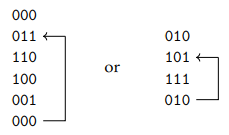
\includegraphics{1x}
\end{center}
Deduce the circuit details by drawing the next-state table and working out 
a minimised sum-of-products expression for the input to each of the three 
state registers ($CBA$). Propose a modification that ensures that in due 
course the circuit will always settle into the cycle shown in the first
pattern. Show a Karnaugh map for each flip-flop input before and after 
your modification, and use them to highlight the change.

The patterns show that this circuit is non-self starting -- and the task is to 
find the circuit which resulted in these two patterns and modify it so that the 
circuit IS self-starting.

Let the state be $CBA$ and the next state as $C'B'A'$.
Combining the next state results for both diagrams gives the following 
three Karnaugh maps for the flip flops.

\begin{center}

{\large $C'$}

\begin{tabular}{|c|c|c|c|c|c|} 
\hline
& & \multicolumn{4}{c|}{$CB$} \\
\hline
& & 00 & 01 & 11 & 10 \\ 
\hline
\multirow{2}{2em}{$A$} 
& 0 & 0 & 1 & 0 & 1 \\
& 1 & 1 & 0 & 1 & 0 \\
\hline
\end{tabular}

From the Karnaugh map:
\begin{equation}
\begin{split}
C' &= CBA + CB\bar A + C\bar BA + \bar CBA\\
C' &= C\oplus B \oplus A\\
\end{split}
\end{equation}

{\large $B'$}

\begin{tabular}{|c|c|c|c|c|c|} 
\hline
& & \multicolumn{4}{c|}{$CB$} \\
\hline
& & 00 & 01 & 11 & 10 \\ 
\hline
\multirow{2}{2em}{$A$} 
& 0 & 0 & 1 & 1 & 1 \\
& 1 & 0 & 0 & 0 & 1 \\
\hline
\end{tabular}

From the Karnaugh map:
\begin{equation}\label{bexpression}
\begin{split}
B' &= C\bar B + B\bar A\\
\end{split}
\end{equation}

{\large $A'$}

\begin{tabular}{|c|c|c|c|c|c|} 
\hline
& & \multicolumn{4}{c|}{$CB$} \\
\hline
& & 00 & 01 & 11 & 10 \\ 
\hline
\multirow{2}{2em}{$A$} 
& 0 & 1 & 1 & 1 & 0 \\
& 1 & 0 & 0 & 1 & 0 \\
\hline
\end{tabular}

From the Karnaugh map:
\begin{equation}
\begin{split}
A' &= CB + \bar C\bar A\\
\end{split}
\end{equation}

\end{center}

I noticed that if FF $B$ only goes to 1 when it is in a state in the first loop, then 
the second loop will go into the first loop and hence the circuit will self-start.
I chose to modify $B$ because it gave the expression which required the least 
modification to the previous expression. This would make it the easiest change.
It was also one of the few modifications that actually reduced the number of gates in 
the expression.

A simple modification that would make the circuit self-start (and hence prevent the second, 
unintended loop) would be changing the expression for $B'$ (\ref{bexpression}) to 

\begin{equation}
\begin{split}
B'' &= C\bar A\\
\end{split}
\end{equation}

This does not affect the first loop, however the circuit now self-starts:
\begin{equation}
\begin{split}
010 &\rightarrow 000\\
101 &\rightarrow 000\\
111 &\rightarrow 101 \rightarrow 000\\
\end{split}
\end{equation}

So the new equation for the next states ($C''B''A''$) is:
\begin{equation}
\begin{split}
C'' &= C\oplus B \oplus A\\
B'' &= C\bar A\\
A'' &= CB + \bar C\bar A\\
\end{split}
\end{equation}

\begin{center}

{\large $C''$}

\begin{tabular}{|c|c|c|c|c|c|} 
\hline
& & \multicolumn{4}{c|}{$CB$} \\
\hline
& & 00 & 01 & 11 & 10 \\ 
\hline
\multirow{2}{2em}{$A$} 
& 0 & 0 & 1 & 0 & 1 \\
& 1 & 1 & 0 & 1 & 0 \\
\hline
\end{tabular}

{\large $B''$}

\begin{tabular}{|c|c|c|c|c|c|} 
\hline
& & \multicolumn{4}{c|}{$CB$} \\
\hline
& & 00 & 01 & 11 & 10 \\ 
\hline
\multirow{2}{2em}{$A$} 
& 0 & 0 & 0 & 1 & 1 \\
& 1 & 0 & 0 & 0 & 0 \\
\hline
\end{tabular}

{\large $A''$}

\begin{tabular}{|c|c|c|c|c|c|} 
\hline
& & \multicolumn{4}{c|}{$CB$} \\
\hline
& & 00 & 01 & 11 & 10 \\ 
\hline
\multirow{2}{2em}{$A$} 
& 0 & 1 & 1 & 1 & 0 \\
& 1 & 0 & 0 & 1 & 0 \\
\hline
\end{tabular}

\end{center}

\item

\begin{enumerate}

\item{Explain (in your own words, no diagrams, bullet points are fine) how 
to modify the simple single cycle processor to permit data memory access.}

Perform the current calculation. Take the result from the ALU and use it to 
address a location in data memory. Then put the result from the memory access 
into a multiplexer with the result straight from the ALU.
The multiplexer then controlls whether the result stored in the register should 
be from memory or the result of the calculation.

\item{Explain (in your own words, no diagrams, bullet points are fine) how 
to modify the simple single cycle processor to permit branching.}

When loading the next result into memory, there is an adder which will increment 
the current address in the program counter. Call this output (a). Put (a) into 
another adder which adds an offset (taken from an instruction decoder). Then 
put this into a MUX with (a) to give the option of branching.

\item{Change two words in order to correct the following sentence: 
\textit{Instruction throughput is usually lower in a multicycle processor 
(compared  to a single cycle processor) and multi-cycle processors make less 
effective use of available chip area}.}

\textit{Instruction throughput is usually \textbf{higher} in a multicycle processor 
(compared  to a single cycle processor) and multi-cycle processors make \textbf{more}
effective use of available chip area}.

\item{Change two words in order to correct the following sentence: \textit{A 
pipelined processor reduces throughput (compared to a multicycle processor) 
and decreases per-instruction latency}}

\textit{A pipelined processor \textbf{increases} throughput (compared to a 
multicycle processor) and \textbf{increases} per-instruction latency}

\end{enumerate}

\item

\begin{examquestion}{2012}{2}{2}

\begin{enumerate}[label=(\alph*)]

\item{With the aid of appropriate diagrams, show how the Source–Drain 
current that flows in a p-channel MOSFET is controlled by the applied 
Gate–Source voltage.}

In a p-channel MOSFET, the Source has a positive voltage. Only if the 
Gate has a lower voltage than the source can current flow (and the transistor turn on).
The transistor is off when the voltage of the gate with respect to the source is $0V$ 
(or positive).\\
When current is flowing, the transistor is on.
This means that a lower voltage in the Gate than in the source turns the transistor on.

\begin{tikzpicture}
\draw[thick,->] (0,0) -- (0,10) node[anchor=north west] {$I_{DS}$};
\draw[thick,->] (0,0) -- (10,0) node[anchor=north] {$V_{DS}$};
\draw[step=1cm,gray,very thin] (0, 0) grid (9.99,9.99);
\draw [black] plot [smooth] coordinates {(0,0) (10, 0)} node[anchor=west] {$V_{GS}=0V$};
\draw [black] plot [smooth] coordinates {(0.0, 0.0)(0.1, 0.07)(0.2, 0.13)(0.3, 0.19)(0.4, 0.25)(0.5, 0.31)(0.6, 0.36)(0.7, 0.42)(0.8, 0.47)(0.9, 0.52)(1.0, 0.57)(1.1, 0.61)(1.2, 0.66)(1.3, 0.7)(1.4, 0.75)(1.5, 0.79)(1.6, 0.83)(1.7, 0.87)(1.8, 0.9)(1.9, 0.94)(2.0, 0.97)(2.1, 1.01)(2.2, 1.04)(2.3, 1.07)(2.4, 1.1)(2.5, 1.13)(2.6, 1.16)(2.7, 1.19)(2.8, 1.21)(2.9, 1.24)(3.0, 1.26)(3.1, 1.29)(3.2, 1.31)(3.3, 1.33)(3.4, 1.36)(3.5, 1.38)(3.6, 1.4)(3.7, 1.42)(3.8, 1.44)(3.9, 1.45)(4.0, 1.47)(4.1, 1.49)(4.2, 1.51)(4.3, 1.52)(4.4, 1.54)(4.5, 1.55)(4.6, 1.57)(4.7, 1.58)(4.8, 1.6)(4.9, 1.61)(5.0, 1.62)(5.1, 1.63)(5.2, 1.65)(5.3, 1.66)(5.4, 1.67)(5.5, 1.68)(5.6, 1.69)(5.7, 1.7)(5.8, 1.71)(5.9, 1.72)(6.0, 1.73)(6.1, 1.74)(6.2, 1.75)(6.3, 1.76)(6.4, 1.76)(6.5, 1.77)(6.6, 1.78)(6.7, 1.79)(6.8, 1.79)(6.9, 1.8)(7.0, 1.81)(7.1, 1.81)(7.2, 1.82)(7.3, 1.82)(7.4, 1.83)(7.5, 1.84)(7.6, 1.84)(7.7, 1.85)(7.8, 1.85)(7.9, 1.86)(8.0, 1.86)(8.1, 1.87)(8.2, 1.87)(8.3, 1.87)(8.4, 1.88)(8.5, 1.88)(8.6, 1.89)(8.7, 1.89)(8.8, 1.89)(8.9, 1.9)(9.0, 1.9)(9.1, 1.9)(9.2, 1.91)(9.3, 1.91)(9.4, 1.91)(9.5, 1.92)(9.6, 1.92)(9.7, 1.92)(9.8, 1.92)(9.9, 1.93)} node[anchor=west] {$V_{GS}=-2V$};
\draw [black] plot [smooth] coordinates {(0.0, 0.0)(0.1, 0.16)(0.2, 0.31)(0.3, 0.45)(0.4, 0.59)(0.5, 0.73)(0.6, 0.85)(0.7, 0.98)(0.8, 1.1)(0.9, 1.21)(1.0, 1.32)(1.1, 1.42)(1.2, 1.52)(1.3, 1.62)(1.4, 1.72)(1.5, 1.8)(1.6, 1.89)(1.7, 1.97)(1.8, 2.05)(1.9, 2.13)(2.0, 2.2)(2.1, 2.27)(2.2, 2.34)(2.3, 2.41)(2.4, 2.47)(2.5, 2.53)(2.6, 2.59)(2.7, 2.64)(2.8, 2.69)(2.9, 2.75)(3.0, 2.8)(3.1, 2.84)(3.2, 2.89)(3.3, 2.93)(3.4, 2.97)(3.5, 3.01)(3.6, 3.05)(3.7, 3.09)(3.8, 3.13)(3.9, 3.16)(4.0, 3.19)(4.1, 3.22)(4.2, 3.25)(4.3, 3.28)(4.4, 3.31)(4.5, 3.34)(4.6, 3.36)(4.7, 3.39)(4.8, 3.41)(4.9, 3.44)(5.0, 3.46)(5.1, 3.48)(5.2, 3.5)(5.3, 3.52)(5.4, 3.54)(5.5, 3.56)(5.6, 3.57)(5.7, 3.59)(5.8, 3.61)(5.9, 3.62)(6.0, 3.64)(6.1, 3.65)(6.2, 3.67)(6.3, 3.68)(6.4, 3.69)(6.5, 3.7)(6.6, 3.71)(6.7, 3.73)(6.8, 3.74)(6.9, 3.75)(7.0, 3.76)(7.1, 3.77)(7.2, 3.78)(7.3, 3.78)(7.4, 3.79)(7.5, 3.8)(7.6, 3.81)(7.7, 3.82)(7.8, 3.82)(7.9, 3.83)(8.0, 3.84)(8.1, 3.84)(8.2, 3.85)(8.3, 3.86)(8.4, 3.86)(8.5, 3.87)(8.6, 3.87)(8.7, 3.88)(8.8, 3.88)(8.9, 3.89)(9.0, 3.89)(9.1, 3.89)(9.2, 3.9)(9.3, 3.9)(9.4, 3.91)(9.5, 3.91)(9.6, 3.91)(9.7, 3.92)(9.8, 3.92)(9.9, 3.92)} node[anchor=west] {$V_{GS}=-4V$};
\draw [black] plot [smooth] coordinates {(0.0, 0.0)(0.1, 0.29)(0.2, 0.57)(0.3, 0.84)(0.4, 1.09)(0.5, 1.33)(0.6, 1.56)(0.7, 1.77)(0.8, 1.98)(0.9, 2.17)(1.0, 2.36)(1.1, 2.54)(1.2, 2.71)(1.3, 2.87)(1.4, 3.02)(1.5, 3.17)(1.6, 3.3)(1.7, 3.44)(1.8, 3.56)(1.9, 3.68)(2.0, 3.79)(2.1, 3.9)(2.2, 4.0)(2.3, 4.1)(2.4, 4.19)(2.5, 4.28)(2.6, 4.36)(2.7, 4.44)(2.8, 4.52)(2.9, 4.59)(3.0, 4.66)(3.1, 4.73)(3.2, 4.79)(3.3, 4.85)(3.4, 4.9)(3.5, 4.96)(3.6, 5.01)(3.7, 5.06)(3.8, 5.1)(3.9, 5.15)(4.0, 5.19)(4.1, 5.23)(4.2, 5.27)(4.3, 5.3)(4.4, 5.34)(4.5, 5.37)(4.6, 5.4)(4.7, 5.43)(4.8, 5.46)(4.9, 5.48)(5.0, 5.51)(5.1, 5.53)(5.2, 5.55)(5.3, 5.58)(5.4, 5.6)(5.5, 5.62)(5.6, 5.64)(5.7, 5.65)(5.8, 5.67)(5.9, 5.69)(6.0, 5.7)(6.1, 5.72)(6.2, 5.73)(6.3, 5.74)(6.4, 5.76)(6.5, 5.77)(6.6, 5.78)(6.7, 5.79)(6.8, 5.8)(6.9, 5.81)(7.0, 5.82)(7.1, 5.83)(7.2, 5.84)(7.3, 5.84)(7.4, 5.85)(7.5, 5.86)(7.6, 5.87)(7.7, 5.87)(7.8, 5.88)(7.9, 5.88)(8.0, 5.89)(8.1, 5.9)(8.2, 5.9)(8.3, 5.91)(8.4, 5.91)(8.5, 5.91)(8.6, 5.92)(8.7, 5.92)(8.8, 5.93)(8.9, 5.93)(9.0, 5.93)(9.1, 5.94)(9.2, 5.94)(9.3, 5.94)(9.4, 5.95)(9.5, 5.95)(9.6, 5.95)(9.7, 5.95)(9.8, 5.96)(9.9, 5.96)} node[anchor=west] {$V_{GS}=-6V$};
\draw [black] plot [smooth] coordinates {(0.0, 0.0)(0.1, 0.52)(0.2, 1.0)(0.3, 1.45)(0.4, 1.87)(0.5, 2.27)(0.6, 2.64)(0.7, 2.98)(0.8, 3.31)(0.9, 3.61)(1.0, 3.89)(1.1, 4.16)(1.2, 4.41)(1.3, 4.64)(1.4, 4.85)(1.5, 5.06)(1.6, 5.25)(1.7, 5.42)(1.8, 5.59)(1.9, 5.75)(2.0, 5.89)(2.1, 6.03)(2.2, 6.15)(2.3, 6.27)(2.4, 6.38)(2.5, 6.49)(2.6, 6.59)(2.7, 6.68)(2.8, 6.76)(2.9, 6.84)(3.0, 6.92)(3.1, 6.99)(3.2, 7.05)(3.3, 7.11)(3.4, 7.17)(3.5, 7.22)(3.6, 7.27)(3.7, 7.32)(3.8, 7.36)(3.9, 7.41)(4.0, 7.44)(4.1, 7.48)(4.2, 7.51)(4.3, 7.54)(4.4, 7.57)(4.5, 7.6)(4.6, 7.63)(4.7, 7.65)(4.8, 7.67)(4.9, 7.69)(5.0, 7.71)(5.1, 7.73)(5.2, 7.75)(5.3, 7.77)(5.4, 7.78)(5.5, 7.8)(5.6, 7.81)(5.7, 7.82)(5.8, 7.83)(5.9, 7.84)(6.0, 7.85)(6.1, 7.86)(6.2, 7.87)(6.3, 7.88)(6.4, 7.89)(6.5, 7.9)(6.6, 7.9)(6.7, 7.91)(6.8, 7.91)(6.9, 7.92)(7.0, 7.92)(7.1, 7.93)(7.2, 7.93)(7.3, 7.94)(7.4, 7.94)(7.5, 7.95)(7.6, 7.95)(7.7, 7.95)(7.8, 7.96)(7.9, 7.96)(8.0, 7.96)(8.1, 7.96)(8.2, 7.97)(8.3, 7.97)(8.4, 7.97)(8.5, 7.97)(8.6, 7.97)(8.7, 7.98)(8.8, 7.98)(8.9, 7.98)(9.0, 7.98)(9.1, 7.98)(9.2, 7.98)(9.3, 7.98)(9.4, 7.98)(9.5, 7.99)(9.6, 7.99)(9.7, 7.99)(9.8, 7.99)(9.9, 7.99)} node[anchor=west] {$V_{GS}=-8V$};
\draw [black] plot [smooth] coordinates {(0.0, 0.0)(0.1, 0.95)(0.2, 1.81)(0.3, 2.59)(0.4, 3.3)(0.5, 3.93)(0.6, 4.51)(0.7, 5.03)(0.8, 5.51)(0.9, 5.93)(1.0, 6.32)(1.1, 6.67)(1.2, 6.99)(1.3, 7.27)(1.4, 7.53)(1.5, 7.77)(1.6, 7.98)(1.7, 8.17)(1.8, 8.35)(1.9, 8.5)(2.0, 8.65)(2.1, 8.78)(2.2, 8.89)(2.3, 9.0)(2.4, 9.09)(2.5, 9.18)(2.6, 9.26)(2.7, 9.33)(2.8, 9.39)(2.9, 9.45)(3.0, 9.5)(3.1, 9.55)(3.2, 9.59)(3.3, 9.63)(3.4, 9.67)(3.5, 9.7)(3.6, 9.73)(3.7, 9.75)(3.8, 9.78)(3.9, 9.8)(4.0, 9.82)(4.1, 9.83)(4.2, 9.85)(4.3, 9.86)(4.4, 9.88)(4.5, 9.89)(4.6, 9.9)(4.7, 9.91)(4.8, 9.92)(4.9, 9.93)(5.0, 9.93)(5.1, 9.94)(5.2, 9.94)(5.3, 9.95)(5.4, 9.95)(5.5, 9.96)(5.6, 9.96)(5.7, 9.97)(5.8, 9.97)(5.9, 9.97)(6.0, 9.98)(6.1, 9.98)(6.2, 9.98)(6.3, 9.98)(6.4, 9.98)(6.5, 9.98)(6.6, 9.99)(6.7, 9.99)(6.8, 9.99)(6.9, 9.99)(7.0, 9.99)(7.1, 9.99)(7.2, 9.99)(7.3, 9.99)(7.4, 9.99)(7.5, 9.99)(7.6, 9.99)(7.7, 10.0)(7.8, 10.0)(7.9, 10.0)(8.0, 10.0)(8.1, 10.0)(8.2, 10.0)(8.3, 10.0)(8.4, 10.0)(8.5, 10.0)(8.6, 10.0)(8.7, 10.0)(8.8, 10.0)(8.9, 10.0)(9.0, 10.0)(9.1, 10.0)(9.2, 10.0)(9.3, 10.0)(9.4, 10.0)(9.5, 10.0)(9.6, 10.0)(9.7, 10.0)(9.8, 10.0)(9.9, 10.0)} node[anchor=west] {$V_{GS}=-10V$};
\end{tikzpicture}

\item

\begin{enumerate}[label=(\roman*)]

\item{Draw the circuit diagram of a NOT gate that comprises an n-channel 
MOSFET and a resistor R.}

\begin{center}
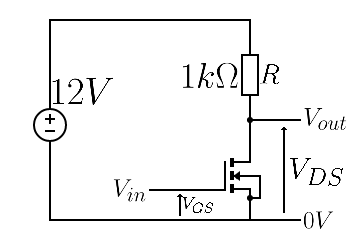
\includegraphics[width=0.5\textwidth]{nmos_inverter}
\end{center}

\item{For the NOT gate in (b)(i), plot the relationship between the input 
voltage, Vin and the output voltage, $V_{out}$. Assume that the power supply 
voltage $V_{DD}$ = 12 V, $R$ = 1 $k\Omega$, and that the MOSFET has the characteristics
given in the following figure.}

\begin{center}
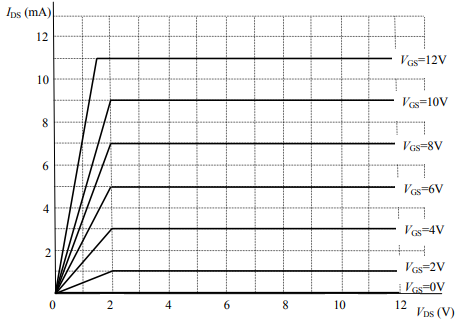
\includegraphics{5bi}
\end{center}

Using the graphical method:

\begin{center}
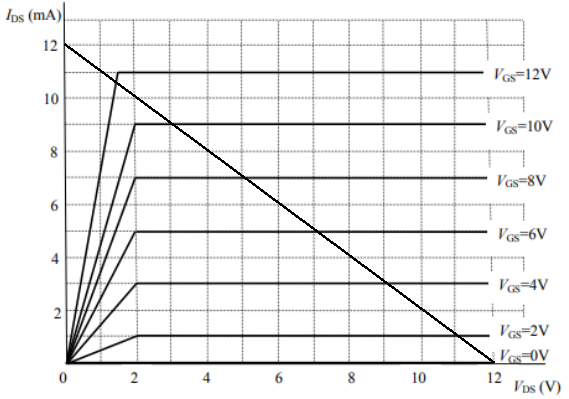
\includegraphics[width=0.8\textwidth]{graphicalmethod}
\end{center}

Plotting $V_{out}$ of the intersections against $V_{GS}$.

\begin{tikzpicture}

\draw[step=1cm,gray,very thin] (0, 0) grid (12.5,12.5);
\draw[thick,->] (0,0) -- (13,0) node[anchor=north west] {$V_{GS}$};
\draw[thick,->] (0,0) -- (0,13) node[anchor=north west] {$V_{DS}$};
\foreach \x in {0,1,2,3,4,5,6,7,8,9,10,11,12}
   \draw (\x cm,1pt) -- (\x cm,-1pt) node[anchor=north] {$\x$};
\foreach \y in {0,1,2,3,4,5,6,7,8,9,10,11,12}
    \draw (1pt,\y cm) -- (-1pt,\y cm) node[anchor=east] {$\y$};
\draw (0,12) node[cross,rotate=0] {};
\draw (2,11) node[cross,rotate=0] {};
\draw (4,9) node[cross,rotate=0] {};
\draw (6,7) node[cross,rotate=0] {};
\draw (8,5) node[cross,rotate=0] {};
\draw (10,3) node[cross,rotate=0] {};
\draw (12,1.5) node[cross,rotate=0] {};
\draw [black] plot [smooth] coordinates {(0,12) (2,11) (4,9) (6,7) (8,5) (10,3) (12,1.5)};

\end{tikzpicture}


\end{enumerate}

\item{For the NOT gate in (b), calculate the power dissipated by the 
entire gate and that by resistor R alone, when $V_{in}$ = 12 V.}

When $V_{in} = 12V$; $V_{GS} = 12V$. Reading off the graph in 3.(b)(ii) gives 
$I_{DS} = 10.6mA$.\\

The voltage across the circuit is $12V$.\\
So using the equation $P=IV$ gives:
\begin{equation}
\begin{split}
P_t &= I_{DS}V_{in}\\
	&= 10.6mA \times 12V\\
	&= 10.6 \times 10^{-3} \times 12\\
	&= 127.2\times 10^{-3}W\\
	&= 127.2mW\\
	&\approx 127mW \text{to 3.S.F}
\end{split}
\end{equation}

So the total power dissipated in the circuit is $\approx 127mW$.

The current flowing through the resistor is $10.6mA$\\
Using the equation for power gives the power dissipated in the resistor is:
\begin{equation}
\begin{split}
P_r &= I^2R\\
	&= 10.6mA^2 \times 1k\Omega\\
	&= 112.36 \times 10^{-6} \times 1 \times 10^{3}\\
	&= 112.36 \times 10^{-3}W\\
	&= 112.36 mW\\
	&\approx 112mW \text{to 3.S.F}\\
\end{split}
\end{equation}

So the power dissipated by resistor R is $\approx 112mW$

\item{The stray capacitance present at the output of the NOT gate in (b) 
can be represented by a capacitor, C = 100 nF connected between the gate 
output and 0 V. Also assume that the MOSFET has an ON resistance Ron = 
100 $\Omega$. The input signal, $V_{in}$, is a 1 kHz square wave with minimum 
and maximum amplitudes of 0 V and 12 V respectively.}

\begin{enumerate}[label=(\roman*)]

\item{Sketch the output signal waveform, Vout, of the NOT gate being sure 
to include indicative rise and fall times and voltage levels.}

Input signal waveform:

\begin{tikzpicture}

\draw[thick,->] (-0.2,-0.2) -- (10.7,-0.2) node[anchor=north] {$t$};
\draw[thick,->] (-0.2,-0.2) -- (-0.2,1.2) node[anchor=south] {$V_{in}/V$};
\draw (-0.15,0) -- (-0.25,0) node[anchor=east] {$0$};
\draw (-0.15,1) -- (-0.25,1) node[anchor=east] {$12$};

\draw (0,0)--(1.5,0)--(1.5,1)--(3,1)--(3,0)--(4.5,0)--(4.5,1)--(6,1)--(6,0)--
(7.5,0)--(7.5,1)--(9,1)--(9,0)--(10.5,0);

\end{tikzpicture}

Output signal waveform:

\begin{tikzpicture}

\draw[thick,->] (-0.2,-0.2) -- (10.7,-0.2) node[anchor=north] {$t$};
\draw[thick,->] (-0.2,-0.2) -- (-0.2,1.2) node[anchor=south] {$V_{out}/V$};
\draw (-0.15,0) -- (-0.25,0) node[anchor=east] {$0$};
\draw (-0.15,1) -- (-0.25,1) node[anchor=east] {$12$};

\draw [black] plot [smooth] coordinates {(0,0) (0.1, 0.181) (0.2, 0.330) (0.3, 0.451) 
(0.4, 0.551) (0.5, 0.632) (0.6, 0.699) (0.7, 0.753) (0.8, 0.798) (0.9, 0.835) 
(1.0, 0.864) (1.1, 0.889) (1.2, 0.909) (1.3, 0.926) (1.4, 0.939) (1.5, 0.950)};
\draw [black] plot [smooth] coordinates {(1.5, 0.950) (1.6, 0.350) (1.7, 0.129) 
(1.8, 0.047) (1.9, 0.017) (2.0, 0.006) (2.1, 0) (2.2, 0) (2.3, 0) (2.4, 0)
(2.5, 0) (2.6, 0) (2.7, 0) (2.8, 0) (2.9, 0) (3, 0)};
\draw [black] plot [smooth] coordinates {(3,0) (3.1, 0.181) (3.2, 0.330) (3.3, 0.451) 
(3.4, 0.551) (3.5, 0.632) (3.6, 0.699) (3.7, 0.753) (3.8, 0.798) (3.9, 0.835) 
(4.0, 0.864) (4.1, 0.889) (4.2, 0.909) (4.3, 0.926) (4.4, 0.939) (4.5, 0.950)};
\draw [black] plot [smooth] coordinates {(4.5, 0.950) (4.6, 0.350) (4.7, 0.129) 
(4.8, 0.047) (4.9, 0.017) (5.0, 0.006) (5.1, 0) (5.2, 0) (5.3, 0) (5.4, 0)
(5.5, 0) (5.6, 0) (5.7, 0) (5.8, 0) (5.9, 0) (6, 0)};
\draw [black] plot [smooth] coordinates {(6,0) (6.1, 0.181) (6.2, 0.330) (6.3, 0.451) 
(6.4, 0.551) (6.5, 0.632) (6.6, 0.699) (6.7, 0.753) (6.8, 0.798) (6.9, 0.835) 
(7.0, 0.864) (7.1, 0.889) (7.2, 0.909) (7.3, 0.926) (7.4, 0.939) (7.5, 0.950)};
\draw [black] plot [smooth] coordinates {(7.5, 0.950) (7.6, 0.350) (7.7, 0.129) 
(7.8, 0.047) (7.9, 0.017) (8.0, 0.006) (8.1, 0) (8.2, 0) (8.3, 0) (8.4, 0)
(8.5, 0) (8.6, 0) (8.7, 0) (8.8, 0) (8.9, 0) (9, 0)};
\draw [black] plot [smooth] coordinates {(9,0) (9.1, 0.181) (9.2, 0.330) (9.3, 0.451) 
(9.4, 0.551) (9.5, 0.632) (9.6, 0.699) (9.7, 0.753) (9.8, 0.798) (9.9, 0.835) 
(10.0, 0.864) (10.1, 0.889) (10.2, 0.909) (10.3, 0.926) (10.4, 0.939) (10.5, 0.950)};
\end{tikzpicture}

\item{How could the rise-time of $V_{out}$ be reduced and what would be the 
impact of your proposed solution on the power dissipation of the circuit?}

The rise-time of $V_{out}$ could be reduced by decreasing the resistance of the 
resistor $R$. This would decrease the time constant $RC$ and so $V_{out}$ would 
rise quicker.\\
But it would increase the power dissipated in the circuit. Since $P=\frac{V^2}{R}$ 
and $V$ is constant: $P\propto\frac{1}{R}$. So a decrease in $R$ will increase the 
power dissipated in the circuit.

\end{enumerate}

\end{enumerate}

\end{examquestion}

\item{A CMOS inverter circuit is shown in part (a) of the figure below. The 
characteristic of the p-type MOSFET T1 is shown in part (b). The 
characteristic of the n-type MOSFET T2 is shown in part (c).}

\begin{enumerate}

\item{Determine the output voltages $V_o$ corresponding to input voltages 
$V_i$ of 0 V and 10 V (low and high inputs).}

When the input voltage, $V_i$ is $0V$: $V_{GS}$ for the PMOS is $-10V$ and $V_{GS}$ 
for the NMOS is $0V$. $V_{out}$ is $10V$.

When the input voltage, $V_i$ is $10V$: $V_{GS}$ for the PMOS is $0V$ and $V_{GS}$ 
for the NMOS is $10V$. $V_{in}$ is $0V$.

\item{Check that the power dissipated in each transistor for high and low 
inputs is negligible.}

When $V_i$ is low: the NMOS is off and the PMOS is on. This means that there 
is not a complete circuit. So current does not flow. Since $P=\frac{I^2}{R}$; and 
$I=0$, the power dissipated is negligible.

When $V_i$ is high: the PMOS is off and the NMOS is on. This means that there is not 
a complete circuit and so current cannot flow. Since $P=\frac{I^2}{R}$; and $I=0$, 
the power dissipated is negligible.

\item{If, due to a faulty lead, the input is floating at becomes +4 V, 
determine $V_o$, the power dissipated in each transistor, and the power 
taken from the supply.}



\begin{center}
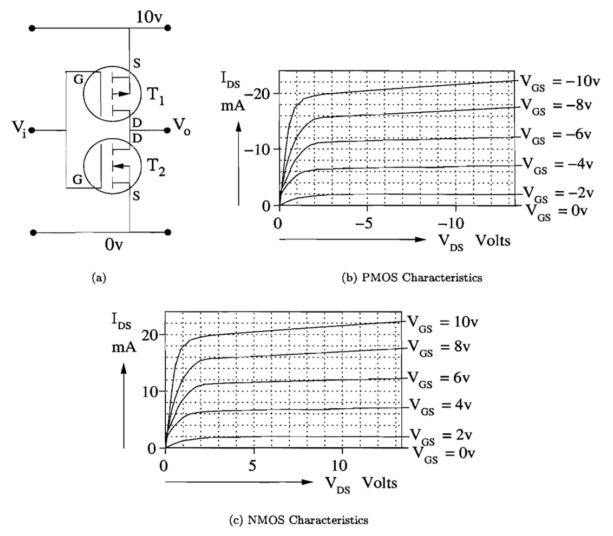
\includegraphics{6c}
\end{center}

If the input is $+4V$, then $V_{GS}$ for the P-MOS is $-6V$ and $V_{GS}$ for the 
N-MOS is $4V$.

So $V_o=6V$. So $V_{DS}$ for the N-MOS is $6V$. On the circuit diagram, this means 
that the current flowing through the N-MOS is $7mA$. So the power dissipated in the N-MOS 
is:
\begin{equation}
\begin{split}
P_{nmos}&=I_{nmos}\times V_{nmos}\\
		&=7mA \times 6V\\
		&=42mW\\
\end{split}
\end{equation}

$V_{DS}$ for the P-MOS is $10V - 6V = 4V$.
Reading off the characteristic graph: at this $V_{DS}$ with a $V_{GS}$ of $-6V$: the current 
flowing through the P-MOS is $11.5mA$. So the power dissipated in the P-MOS is:
\begin{equation}
\begin{split}
P_{nmos}&=I_{pmos}\times V_{pmos}\\
		&=11.5mA \times 4V\\
		&=46mW\\
\end{split}
\end{equation}

The power taken from the supply is equal to the sum of the power dissipated across both of 
the transistors.
\begin{equation}
\begin{split}
P_{supply}&=P_{nmos} + V_{pmos}\\
		&=42mW + 46mW\\
		&=88mW\\
\end{split}
\end{equation}

\end{enumerate}

\item{Find and sketch $V(t)$ in the following circuit (start from first 
principles, i.e. Kirchoff’s laws, Ohm’s law, the definition of capacitance, 
current, etc.):}

\begin{center}
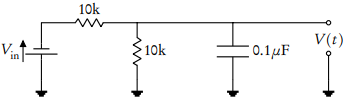
\includegraphics{7x}
\end{center}

V(t) measures the voltage across the $0.1\mu F$ capacitor.

Initially, the upper $10k\Omega$ resistor dominates the resistance in the circuit. 
So initially the voltage across the capacitor is $0V$. As the capacitor charges up, 
the voltage across it will increase. However, since there are two resistors and the 
capacitor is only in parallel with one of them: the voltage across the capacitor will never 
exceed the voltage across the second resistor.\\
Using the potential divider equation: 
\begin{equation}
\begin{split}
V_{max} &= V_{in} \times \frac{10k\Omega}{10k\Omega + 10k\Omega}\\
		&= V_{in} \times \frac{1}{2}\\
		&= \frac{V_{in}}{2}\\
\end{split}
\end{equation}

So the capacitor starts at $0V$ and charges to a maximum of $\frac{V_{in}}{2}$. 

Using the equation for a charging capacitor:
\begin{equation}
\begin{split}
V &= V_0(1 - e^{-\frac{t}{\tau}})\\
  &= V_0(1 - e^{-\frac{t}{RC}})\\
  &= V_0(1 - e^{-\frac{t}{10k\Omega 0.1\mu F}})\\
  &= V_0(1 - e^{-\frac{t}{1ms}})\\
\text{Substituting this}&\text{ into the previous equation gives:}\\
V &= \frac{V_{in}}{2}(1 - e^{-\frac{t}{1ms}})
\end{split}
\end{equation}

\textbf{Add actual times onto this. You know RC so can do that.\\
This graph contains times up to 5RC.}

V(t) is the voltagea across the capacitor. So the question is asking us to plot a graph of the 
voltage across the capacitor.\\

\begin{tikzpicture}

\draw[step=0.5,lightgray,ultra thin] (0, 0) grid (11.25,7.25);

\draw[thick,->] (0,0) -- (11.52,0) node[anchor=west] {$t/ms$};
\draw[thick,->] (0,0) -- (0,7.5) node[anchor=south] {$V(t)/V$};
\draw[thick] (0.1,0) -- (-0.1,0) node[anchor=east] {$0$};
\draw[thick] (0.1,7) -- (-0.1,7) node[anchor=east] {$\frac{V_{in}}{2}$};
\draw[thick] (0,0.1) -- (0,-0.1) node[anchor=north] {$0$};
\draw[thick] (2.2, 0.1) -- (2.2, -0.1) node[anchor=north] {$1$};
\draw[thick] (4.4, 0.1) -- (4.4, -0.1) node[anchor=north] {$2$};
\draw[thick] (6.6, 0.1) -- (6.6, -0.1) node[anchor=north] {$3$};
\draw[thick] (8.8, 0.1) -- (8.8, -0.1) node[anchor=north] {$4$};
\draw[thick] (11, 0.1) -- (11, -0.1) node[anchor=north] {$5$};

\draw [black] plot [smooth] coordinates {(0.0, 0.0) (0.22, 0.67) 
(0.45, 1.27) (0.67, 1.81) (0.9, 2.31) (1.12, 2.75) (1.35, 3.16) (1.57, 3.52) 
(1.8, 3.85) (2.02, 4.15) (2.25, 4.42) (2.47, 4.67) (2.7, 4.89) (2.92, 5.09) 
(3.15, 5.27) (3.37, 5.44) (3.6, 5.59) (3.82, 5.72) (4.05, 5.84) (4.27, 5.95) 
(4.5, 6.05) (4.72, 6.14) (4.95, 6.22) (5.17, 6.3) (5.4, 6.36) (5.62, 6.43) 
(5.85, 6.48) (6.07, 6.53) (6.3, 6.57) (6.52, 6.61) (6.75, 6.65) (6.97, 6.68) 
(7.2, 6.71) (7.42, 6.74) (7.65, 6.77) (7.87, 6.79) (8.1, 6.81) (8.32, 6.83) 
(8.55, 6.84) (8.77, 6.86) (9.0, 6.87) (9.22, 6.88) (9.45, 6.9) (9.67, 6.91) 
(9.9, 6.91) (10.12, 6.92) (10.35, 6.93) (10.57, 6.94) (10.8, 6.94) (11.02, 6.95) 
(11.25, 6.95)};

\end{tikzpicture}

\end{enumerate}

\vspace{1cm}

The two questions which were removed from the supervision work are included below.

\vspace{1cm}

\begin{enumerate}

\item{For the following circuit}

\begin{center}
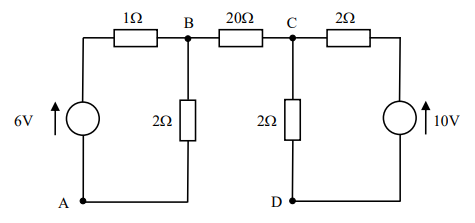
\includegraphics{2.22}
\end{center}

\begin{enumerate}

\item{What is the current flowing through the $20\Omega$ resistor?}

The current flowing through the $20\Omega$ resistor is $0A$.\\
This is because although the two circuits are connected, they do not have 
a route back. So if there was a current flowing through the $20\Omega$ 
resistor then one cell would have a greater current flowing 
out than in and the other cell would have a lower current flowing out 
than in. Which would violate Kirchoff’s $1^{st}$ law.

\item{Find the voltage at nodes B, C, and D with respect to node A, i.e., 
$V_{AB}$, $V_{AC}$ and $V_{AD}$.}

\begin{enumerate}
\item[($V_{AB}$)] Since there is no current flowing through the $20\Omega$ resistor, we can 
consider the left hand circuit as a separate circuit when considering $V_{AB}$.

The total resistance of the left hand circuit is $3\Omega$ ($1\Omega + 2\Omega$).\\
The voltage supplied to the left hand circuit is $6V$.\\
So using Ohm's Law:
\begin{equation}
\begin{split}
V &= IR\\
I &= \frac{V}{R}\\
I &= \frac{6V}{3\Omega}\\
I &= 2A\\
\end{split}
\end{equation}

Since we are considering $V_{AB}$, we must consider the reverse voltage over the 
$2\Omega$ resistor. So $V_{AB}$ = - $V_{R_{2\Omega}}$.
\begin{equation}
\begin{split}
V_{R_{2\Omega}} &= IR\\
 &= 2A \times 2\Omega\\
 &= 4V\\
V_{AB} &= - V_{R_{2\Omega}}\\
\therefore V_{AB} &= -4V\\
\end{split}
\end{equation}

\item[($V_{AC}$)] There are no components between $A$ and the LHS Cell. So 
the voltage at $A$ is $0V$. The voltage $V_{AC}$ is 
the voltage at $A$ minus the voltage at $C$. This is equivalent to the negative 
of the voltage at $C$.

In the right-hand circuit:
\begin{equation}
\begin{split}
V &= IR\\
I &= \frac{V}{R}\\
I &= \frac{10V}{2\Omega + 2\Omega}\\
I &= \frac{5}{2}A\\
V_{CD} &= IR\\
V_{CD} &= \frac{5}{2}A \times 2\Omega\\
V_{CD} &= 5V\\
V_{AC} &= - V_{CD}\\
\therefore V_{AC} &= - 5V\\
\end{split}
\end{equation}

\item[($V_{AD}$)] There are no components between $D$ and the battery. So the voltage 
at $D$ is $0V$. Since the voltage at $A$ is also $0V$; The voltage at $D$ with respect to 
$A$ is $0V$.\\ $\therefore V_{AD} = 0V$.

\end{enumerate}
\end{enumerate}

\item{The op-amp based amplifiers shown in Fig. 2 (a) and (b) are used to 
boost the +/- 100mV signal at the output of a transducer so that suits the 
+/- 5V input voltage range of an analogue to digital converter (ADC).}

\begin{center}
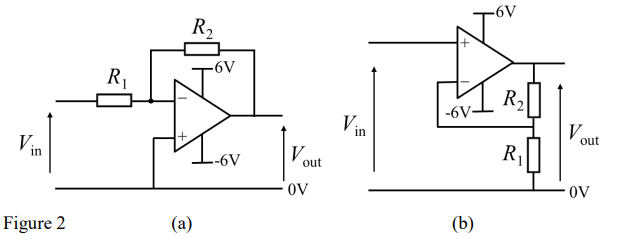
\includegraphics{3.25}
\end{center}

\begin{enumerate}

\item{What voltage gain is required?}

In the first circuit (Fig. 2 (a) -- an inverting amplifier); the voltage gain needs to be $-5.1V$.\\
The second equation (Fig. 2 (b) -- a non-inverting amplifier); the voltage gain required is $4.9V$.

\item{For the inverting and non-inverting amplifiers in Fig. 2 (a) and (b) 
respectively, select the value of $R_2$ if $R_1 = 1k\Omega$.}

The formula for the output voltage from an inverting amplifier (such as in Fig. 2 (a)) is:
\begin{center}
\begin{equation}
\begin{split}
\frac{V_{out}}{V_{in}} &= -\frac{R_2}{R_1}\\
\end{split}
\end{equation}
Given that $V_{out} = -5V$, $V_{in} = 100mV$ and $R_1 = 1k\Omega$:
\begin{equation}
\begin{split}
\frac{V_{out}}{V_{in}} &= -\frac{R_2}{R_1}\\
\frac{-5V}{0.1V} &= -\frac{R_2}{1k\Omega}\\
-50 \times 1k\Omega &= -R_2\\
50k\Omega &= R_2\\
\end{split}
\end{equation}
So the value of $R_2$ in Fig. 2 (a) is $50k\Omega$.
\end{center}

The formula for the output voltage from a non-inverting amplifier (such as in Fig. 2 (b)) is:
\begin{center}
\begin{equation}
\begin{split}
\frac{V_{out}}{V_{in}} &= 1 + \frac{R_2}{R_1}\\
\end{split}
\end{equation}
Given that $V_{out} = -5V$, $V_{in} = 100mV$ and $R_1 = 1k\Omega$:
\begin{equation}
\begin{split}
\frac{V_{out}}{V_{in}} &= 1 + \frac{R_2}{R_1}\\
\frac{5V}{0.1V} &= 1 + \frac{R_2}{1k\Omega}\\
50k\Omega &= 1k\Omega + R_2\\
49k\Omega &= R_2\\
\end{split}
\end{equation}
So the value of $R_2$ in Fig. 2 (b) is $49k\Omega$.
\end{center}

\item{What problem arises if the transducer output voltage exceeds $+/-120mV$?}

An op-amp scales up the input by a given factor.\\
For this specific op-amp, that factor is 50$\times$. However, the maximum voltage which 
it can output is limited by the supply voltage. The supply voltage for this 
op-amp is $+/-6V$. So the maximum ouput voltage from these op-amps is $+/-6V$. 
If the transducer output voltage (which is the op-amps input) is greater 
than $+/-120mV$, then the voltage which the op-amp \textit{should} output 
(the transducer output voltage $\times$ 50) is greater than $+/-6V$ so 
the op-amp cannot output that high a voltage. So the voltage output by the 
op-amp is not the right voltage.\\
IE if the transducer output voltage was $200mV$, then the op-amp output voltage 
should be $10V$. However, it will only output $6V$.

In short: if the transducer output voltage exceeds $+/-120mV$, the voltage of the 
power supply is too low and prevents the op-amp from outputting the appropriate voltage.

\end{enumerate}

\end{enumerate}
\end{document}